% Companion verification: Python package `quantum_foundations.sedenion`, notebooks in
% `papers/sedenion-associator-probe/notebooks/`, companion map in `COMPANION.md`.
% !LW recipe=paper build.sh (echo 1/4..4/4)
\pdfoutput=1
\documentclass[12pt,a4paper]{article}
\usepackage[margin=1in]{geometry}
\usepackage{amsmath,amssymb,amsthm,mathtools}
\usepackage{graphicx}
\usepackage{booktabs}
\usepackage{enumitem}
\usepackage{placeins}
\usepackage[hidelinks]{hyperref}
\usepackage{xurl}
\usepackage{xcolor}
\usepackage{tikz}
\usetikzlibrary{positioning}

\newtheorem{theorem}{Theorem}[section]
\newtheorem{lemma}[theorem]{Lemma}
\newtheorem{proposition}[theorem]{Proposition}
\newtheorem{definition}[theorem]{Definition}
\newtheorem{remark}[theorem]{Remark}
\newtheorem{corollary}[theorem]{Corollary}

\title{Sedenion associator probe decomposition of the octonion generation graph:\\ a combinatorial stratification of $\mathrm{Im}(\mathbb{S})$ over Fano lines}
\author{Bart{\l}omiej Rosa}
\date{v1.0 (\today)}

\begin{document}
\maketitle

\begin{abstract}
We establish that the eight Cayley--Dickson sedenion basis probes $\{e_8, \ldots, e_{15}\}$, when used as external probes of the imaginary octonions $\mathrm{Im}(\mathbb{O})$ via associator norm matrices, partition into four characteristic-polynomial classes with multiplicities $(1, 3, 3, 1)$, and this partition is uniform across all 28 configurations $(L_0, (g_1, g_2, g_3))$ parameterized by 7 Fano lines and $\binom{4}{3} = 4$ complementary ordered triples. Concretely, fix a Fano line $L_0 \subset \{1, \ldots, 7\}$ and an ordered triple $(g_1, g_2, g_3)$ of distinct complementary directions; for each $k \in \{8, \ldots, 15\}$ form the $3 \times 3$ matrix $A^{(k)}_{ij} = \|[e_{g_i}, e_{g_j}, e_k]\|$, where $[\cdot, \cdot, \cdot]$ is the associator and $\|\cdot\|$ the Cayley--Dickson norm. We prove (i) zero diagonal, (ii) entries in $\{0, 2\}$, (iii) characteristic-polynomial classification with eigenvalues $\{4, -2, -2\}$, $\{2, 0, -2\}$, $\{2\sqrt{2}, 0, -2\sqrt{2}\}$, $\{0, 0, 0\}$ (classes Democratic, Edge, Hub, Zero respectively), and (iv) a deterministic probe-to-class mapping from $k$ alone, whose Edge component realizes a canonical bijection $L_0 \to E(K_3)$ with the edges of the generation triangle. The classification is $G_2$-invariant, where $G_2 = \mathrm{Aut}(\mathbb{O})$ acts on $\mathbb{S}$ by the canonical lift of $\mathbb{O}$-automorphisms along Cayley--Dickson doubling (the $G_2$ factor of $\mathrm{Aut}(\mathbb{S}) = G_2 \times S_3$). Proofs are closed-form case analyses on Fano incidence.
\end{abstract}

\tableofcontents

\section{Introduction}
The Cayley--Dickson doubling chain
\[
\mathbb{R}\subset \mathbb{C}\subset \mathbb{H}\subset \mathbb{O}\subset \mathbb{S}
\]
produces the octonions $\mathbb{O}$, the last normed division algebra, and the sedenions $\mathbb{S}$, the first algebra with zero divisors \cite{Schafer1966,ConwaySmith2003,Cawagas2004}.
The octonions carry exceptional combinatorics: the seven imaginary units $\{e_1,\dots,e_7\}$ form the \emph{Fano plane} of quaternionic lines \cite{Baez2002}.

\medskip
\noindent\textbf{Question.}
The doubling $\mathbb{O}\to\mathbb{S}$ destroys alternativity, so sedenions are often treated as ``too degenerate'' for rigid structure.
Nevertheless, does the sedenion associator reveal hidden organization in $\mathrm{Im}(\mathbb{O})$ when used as an \emph{external probe}?

\medskip
\noindent\textbf{Answer (informal).}
For the matrices $A^{(k)}$ defined above, the eight probes split into four characteristic-polynomial classes (Democratic, Edge, Hub, Zero), with multiplicities $1+3+3+1$.
Moreover, the Edge and Hub classes align with the edges and vertex stars of the complete graph $K_3$ on the three complementary directions.
We use the term ``generation graph'' in a strictly graph-theoretic sense: the complete graph $K_3$ on the three complementary directions $(g_1, g_2, g_3)$, which we also call the \emph{complementary triple triangle}. The term is not intended to overlap with two existing usages to which the reader may otherwise reach: (i) the ``generating graph'' $\Gamma(G)$ of a finite group~\cite{burness_guralnick_harper2018} (vertices: non-identity elements; edges: pairs generating $G$), a distinct combinatorial object studied in algebraic graph theory; and (ii) the physics notion of three fermion generations in division-algebra constructions~\cite{Furey2018,gresnigt2019,gresnigt2023,gourlay_gresnigt2024}. The paper is purely algebraic--combinatorial and makes no phenomenological claims (cf.~\S\ref{sec:nonclaims}). Wherever a more neutral term is desired, the reader may substitute ``the complete graph $K_3$ on the complementary triple $(g_1, g_2, g_3)$'' throughout.

\medskip
\noindent\textbf{Physical context (one paragraph only).}
Several authors connect division algebras to Standard Model flavor structures \cite{Dixon1994book,Furey2018,Boyle2020}.
Our main theorems are \emph{purely algebraic}; we do not claim a physical realization of sedenions as an internal symmetry algebra.

\subsection{Reader's guide}
Section~\ref{sec:prelim} fixes notation for Cayley--Dickson doubling, recalls the Fano plane, and defines sedenion probes.
Section~\ref{sec:main} states the main lemmas and theorems.
Section~\ref{sec:graph} interprets the result as a $K_3$ decomposition.
Section~\ref{sec:discuss} discusses literature, limitations, and open problems.
Appendices~\ref{app:mult} and~\ref{app:configs} record the octonion multiplication table and the full $28$-configuration probe-to-class assignment.

\section{Preliminaries}\label{sec:prelim}

\subsection{Cayley--Dickson doubling}\label{subsec:cd}
Let $A$ be a finite-dimensional real algebra with conjugation $a\mapsto \bar a$ satisfying $\overline{ab}=\bar b\,\bar a$.
The Cayley--Dickson double $A'$ consists of pairs $(a,b)$ with product
\begin{equation}\label{eq:cd-doubling}
(a,b)(c,d)=(ac-\bar d\,b,\; da+b\bar c),
\end{equation}
and conjugation $(a,b)^*=(\bar a,-b)$.

\begin{remark}[Doubling conventions and labelling-independence]
\label{rem:doubling}
There are eight Cayley--Dickson doubling products up to isomorphism~\cite{bales2017}; all eight produce isomorphic normed division algebras through level 3 (the standard octonions $\mathbb{O} = \mathbb{A}_3$), and zero divisors enter uniformly at level 4 ($\mathbb{A}_4 = \mathbb{S}$). The amended v4 (2023) of the arXiv companion tightens the sign analysis in the elimination table (Table~8.1) but does not change the count. We adopt the convention $(a, b)(c, d) = (ac - \bar{d}b, \, da + b\bar{c})$ used in~\cite[\S6.1]{ConwaySmith2003} and apply it consistently throughout.

The results of \S\ref{sec:main} are labelling-independent in the following precise sense. The $480$ real octonion multiplication tables (Corollary~\ref{cor:g2-invariance}) are related to each other by $G_2 = \mathrm{Aut}(\mathbb{O})$ combined with the discrete group of basis relabellings (sign flips and permutations of $\{e_1, \ldots, e_7\}$ preserving Fano incidence). Under any such relabelling:
\begin{enumerate}[label=(\alph*)]
    \item the four spectral classes (Democratic, Edge, Hub, Zero) and their multiplicities $(1, 3, 3, 1)$ are preserved as a \emph{set partition} of the $224$-element configuration space $\{(L_0, (g_1, g_2, g_3), k)\}$; this is the genuine consequence of Corollary~\ref{cor:g2-invariance};
    \item the specific probe-to-class map $k \mapsto \text{class}(k)$ is preserved only up to the permutation of probe indices induced by the relabelling.
\end{enumerate}
The tabulation in Appendix~\ref{app:configs} and the computational verification use the specific labelling adopted above; (a) holds universally, while (b) is the specific realisation of that universal pattern in our labelling.
\end{remark}
We identify $a\in A$ with $(a,0)$ and write $\varepsilon=(0,1)$ so that $A'=A\oplus A\varepsilon$.

\begin{definition}[Standard basis via iterated doubling]
Starting from $e_0=1\in\mathbb{R}$, iterating doubling produces basis vectors $\{e_0,\dots,e_{2^n-1}\}$ at level $n$.
We write $\mathbb{S}$ for $n=4$ (sedenions) with basis $\{e_0,\dots,e_{15}\}$.
\end{definition}

\begin{remark}[Power-associativity]
Every Cayley--Dickson algebra is \emph{power-associative}: $[x,x,y]=0$ for all $x,y$, where the associator is
\begin{equation}\label{eq:assoc-def}
[x,y,z]:=(xy)z-x(yz).
\end{equation}
We use this only through the identity $[e_i,e_i,e_k]=0$ for basis elements.
\end{remark}

\subsection{Octonions and the Fano plane}
We use the same Cayley--Dickson basis for $\mathbb{O}$ as in Appendix~\ref{app:mult}.

\begin{definition}[Fano line]
A \emph{Fano line} is a triple $\{a,b,c\}\subset\{1,\dots,7\}$ of distinct indices such that, after choosing signs if needed,
$e_ae_b=\pm e_c$ cyclically.
\end{definition}

\begin{proposition}[Seven lines]\label{prop:fano}
There are exactly seven Fano lines; they form the classical Fano plane incidence structure \cite{Baez2002}.
Each unordered pair $\{i,j\}\subset\{1,\dots,7\}$ lies on a unique line, and each index lies on three lines.
\end{proposition}

\begin{definition}[Complement of a line]
Given a Fano line $L_0=\{a,b,c\}$, define $\mathrm{Comp}(L_0)=\{1,\dots,7\}\setminus L_0$, which has cardinality $4$.
\end{definition}

\subsection{Sedenions and probes}
Write $\mathbb{S}=\mathbb{O}\oplus \mathbb{O}\ell$ with $\ell^2=-1$ the doubling generator; in basis notation, $e_{8+i}$ corresponds to $(0,e_i)$ for $i=0,\dots,7$.
Indices $0,\dots,7$ are the ``octonionic half''; indices $8,\dots,15$ are the ``sedenionic half''.

\begin{definition}[Associator probe matrices]
Fix a Fano line $L_0$, choose an ordered triple $(g_1,g_2,g_3)$ of three distinct elements of $\mathrm{Comp}(L_0)$, and fix $k\in\{8,\dots,15\}$.
Define $A^{(k)}\in\mathbb{R}^{3\times 3}$ by
\begin{equation}\label{eq:Adef}
A^{(k)}_{ij}:=\bigl\|[e_{g_i},e_{g_j},e_k]\bigr\|,
\end{equation}
where $\|x\|:=\sqrt{x\bar x}$ is the Cayley--Dickson norm (Euclidean length in the standard basis).
\end{definition}

\begin{remark}[Probes in the octonion half]
\label{rem:octonion-half}
The restriction to $k \in \{8, \ldots, 15\}$ (the sedenionic half) is essential: for $k \in \{0, \ldots, 7\}$ the probe $e_k$ lies in $\mathbb{O}$, so the associator $[e_{g_i}, e_{g_j}, e_k]$ is computed entirely within $\mathbb{O}$ and falls under the classical Fano/non-Fano dichotomy for octonion basis triples. Such probes contribute no information beyond the well-known associator structure of $\mathrm{Im}(\mathbb{O})$ and are omitted from the analysis below.
\end{remark}

\section{Main results}\label{sec:main}

\begin{proposition}[Cross-level associator formula]
\label{prop:cross-assoc}
For any $p, q, f \in \mathbb{O}$, in $\mathbb{S} = \mathbb{O} \oplus \mathbb{O}\ell$,
\[
  [(p,0),\,(q,0),\,(0,f)]_{\mathbb{S}} = \bigl(0,\ f\cdot(pq) - (f q)\, p\bigr),
\]
where all products on the right are computed in $\mathbb{O}$.
\end{proposition}

\begin{proof}
Applying \eqref{eq:cd-doubling},
\[
  (p,0)(q,0) = (pq, 0), \quad
  (pq,0)(0,f) = (0, f\,(pq)),
\]
\[
  (q,0)(0,f) = (0, fq), \quad
  (p,0)(0, fq) = (0, (fq)p).
\]
Subtracting gives the claim.
\end{proof}

\begin{definition}[Symmetric associator]
For $x, y, z$ in any non-associative algebra define
$S(x,y,z) := (xy)z + x(yz).$
\end{definition}

\begin{lemma}[Reduction to symmetric associator]
\label{lem:reduction-to-S}
For distinct $p, q \in \mathrm{Im}(\mathbb{O}) \cap \{e_1,\ldots,e_7\}$ and any $f \in \mathbb{O}$,
\[
  [(p,0),(q,0),(0,f)]_{\mathbb{S}} = \bigl(0,\ -\,S(f, q, p)\bigr).
\]
\end{lemma}

\begin{proof}
Since $p, q$ are distinct imaginary basis units, $pq = -qp$, hence $f(pq) = -f(qp)$ and
$f(pq) - (fq)p = -\bigl(f(qp) + (fq)p\bigr) = -S(f,q,p)$.
Combine with Proposition~\ref{prop:cross-assoc}.
\end{proof}

\begin{lemma}[Zero diagonal]\label{lem:diag0}\label{lem:zero-diagonal}
For all $i\in\{1,2,3\}$ and all probes $k\in\{8,\dots,15\}$, $A^{(k)}_{ii}=0$.
\end{lemma}

\begin{proof}
Apply Proposition~\ref{prop:cross-assoc} with $p = q = e_{g_i}$ and $f \in \mathbb{O}$
such that $e_k = (0, f)$:
\[
  [e_{g_i},\, e_{g_i},\, e_k] = \bigl(0,\ f \cdot e_{g_i}^{\,2} - (f \cdot e_{g_i}) \cdot e_{g_i}\bigr)
  = \bigl(0,\ -f - (f \cdot e_{g_i}) \cdot e_{g_i}\bigr).
\]
The right alternative law in $\mathbb{O}$ gives $(f \cdot e_{g_i}) \cdot e_{g_i} = f \cdot e_{g_i}^{\,2} = -f$,
so the second component vanishes.
Note that $\mathbb{S}$ is \emph{not} globally alternative. The elements involved --- the imaginary basis unit $e_{g_i}$ with $g_i \in \{1, \ldots, 7\}$ and the element $f \in \mathrm{Im}(\mathbb{O})$ --- both lie in $\mathbb{O} \subset \mathbb{S}$, so the calculation $(f \cdot e_{g_i}) \cdot e_{g_i} = f \cdot e_{g_i}^2 = -f$ is an identity in $\mathbb{O}$, where the right alternative law $(yx)x = yx^2$ holds. Artin's theorem~\cite[\S III.2]{Schafer1966} gives the general statement that any two elements of an alternative algebra generate an associative subalgebra, and~\cite[\S3--4]{Cawagas2004} describes the explicit subalgebra structure of $\mathbb{S}$; we invoke here only the immediate fact that the octonion half $\mathbb{O} \subset \mathbb{S}$ is itself alternative.
\end{proof}

\begin{lemma}[Symmetry]
\label{lem:symmetry}
For all configurations $(L_0, (g_1, g_2, g_3))$ and all $k \in \{8, \ldots, 15\}$, the matrix $A^{(k)}$ is symmetric: $A^{(k)}_{ij} = A^{(k)}_{ji}$.
\end{lemma}

\begin{proof}
The associator $[x, y, z] = (xy)z - x(yz)$ in any non-associative algebra satisfies $[y, x, z] = -[x, y, z]$ when $\{x, y\}$ is a pair of anti-commuting elements. For distinct imaginary basis units $e_{g_i}, e_{g_j} \in \mathrm{Im}(\mathbb{O})$, we have $e_{g_j} e_{g_i} = -e_{g_i} e_{g_j}$, so $[e_{g_j}, e_{g_i}, e_k]_{\mathbb{S}} = -[e_{g_i}, e_{g_j}, e_k]_{\mathbb{S}}$, and the norms agree: $A^{(k)}_{ji} = \|[e_{g_j}, e_{g_i}, e_k]\| = \|[e_{g_i}, e_{g_j}, e_k]\| = A^{(k)}_{ij}$. The diagonal case $i = j$ is Lemma~\ref{lem:zero-diagonal}.
\end{proof}

\begin{lemma}[Non-Fano anti-associativity]
\label{lem:non-fano-anti-assoc}
Let $e_m, e_b, e_a$ be three distinct imaginary basis units of $\mathbb{O}$ with $m, a, b \in \{1, \ldots, 7\}$. If $\{m, b, a\}$ is not a Fano line, then
\[
  (e_m e_b)\, e_a \;=\; -\,e_m (e_b\, e_a).
\]
Equivalently, the symmetric associator vanishes: $S(e_m, e_b, e_a) = 0$.
\end{lemma}

\begin{proof}
On imaginary basis units of $\mathbb{O}$, the associator $[\cdot, \cdot, \cdot]$ is totally antisymmetric, a consequence of the alternative laws $[x,x,y] = 0$ and $[y,x,x] = 0$ applied by linearization~\cite[\S~1.1]{Baez2002}\cite[Ch.~III]{Schafer1966}. On distinct imaginary basis units, the associator is therefore an alternating trilinear form.

Assume $\{m, b, a\}$ is not a Fano line. Then $\{e_m, e_b, e_a\}$ does not lie in a common quaternion subalgebra of $\mathbb{O}$. In the Fano plane $\mathrm{PG}(2, 2)$, the three pairs $\{m, b\}, \{b, a\}, \{m, a\}$ each determine a unique Fano line, and these three lines are distinct (since $\{m, b, a\}$ is not collinear). The three associated third-points together with $\{m, b, a\}$ form a set of six points of $\mathrm{PG}(2, 2)$; the unique seventh point $d$ is the \emph{fourth point of the associator quadrangle}. By a standard finite calculation on the octonion multiplication table (equivalently, the associative $3$-form identification of~\cite[\S 2.2]{Baez2002}),
\[
[e_m, e_b, e_a]_{\mathbb{O}} = \pm 2 \, e_d,
\]
a non-zero signed basis element of norm $2$.

Set $u := (e_m e_b) e_a$ and $v := e_m (e_b e_a)$. Each is a signed basis element of $\mathbb{O}$ (the product of two basis elements in $\mathbb{O}$ is $\pm e_k$ for some $k$), so $\|u\| = \|v\| = 1$. By definition of the associator,
\[
  u - v \;=\; [e_m, e_b, e_a]_\mathbb{O},
\]
so by the preceding paragraph $\|u - v\| = 2$, i.e., $\|u - v\|^2 = 4$. Expanding, $\|u\|^2 - 2\langle u, v\rangle + \|v\|^2 = 4$, giving $\langle u, v\rangle = -1$. By the following elementary fact: for unit vectors $u, v$ in any Euclidean space, if $\|u - v\|^2 = 4$ then $u = -v$ (equality case in the Cauchy--Schwarz inequality). Applied to the Euclidean structure on $\mathbb{R}^8 \cong \mathbb{O}$, this gives $u = -v$ in our setting. Therefore
\[
  (e_m e_b) e_a \;=\; u \;=\; -v \;=\; -e_m(e_b e_a),
\]
and equivalently $S(e_m, e_b, e_a) = u + v = 0$.
\end{proof}

\begin{lemma}[Entry quantization]\label{lem:quant}
For all configurations $(L_0,(g_1,g_2,g_3))$ in the finite family of Section~\ref{sec:prelim} and all $i,j,k$,
$A^{(k)}_{ij}\in\{0,2\}$.
\end{lemma}

\begin{proof}[Proof of Lemma~\ref{lem:quant}]
By Lemma~\ref{lem:reduction-to-S},
$A^{(8+m)}_{pq} = \|S(e_m, e_{g_q}, e_{g_p})\|_{\mathbb{O}}$
for $p \neq q$, where $m = k - 8$.
Fix distinct $p,q\in\{1,2,3\}$ and write $a:=g_p$, $b:=g_q$ for the corresponding complementary indices.

\textbf{Case A} ($m = 0$). $S(1, e_b, e_a) = e_b e_a + e_b e_a = 2 e_b e_a$, norm $2$.

\textbf{Case B} ($m = a$). The chain proceeds by three named identities, applied in turn:
\begin{itemize}
    \item flexibility: $(e_a e_b) e_a = e_a (e_b e_a)$, so $S(e_a, e_b, e_a) = 2 \, e_a (e_b e_a)$;
    \item anticommutativity of distinct imaginary basis units: $e_b e_a = -e_a e_b$, so $2 \, e_a (e_b e_a) = -2 \, e_a (e_a e_b)$;
    \item left alternative law $(xx) y = x(xy)$: $-2 \, e_a (e_a e_b) = -2 (e_a e_a) e_b = 2 e_b$, using $e_a^2 = -1$.
\end{itemize}
Norm $2$.

\textbf{Case C} ($m = b$). Similarly
$S(e_b, e_b, e_a) = (e_b e_b)e_a + e_b(e_b e_a) = -e_a - e_a = -2 e_a$,
using the alternative identity. Norm $2$.

\textbf{Case D} ($m \in \{1,\ldots,7\}$, $m,a,b$ all distinct). We split on Fano incidence.

\emph{Case D1}: $\{m, a, b\}$ is a Fano line. Then $\{e_m, e_a, e_b\}$ generates a quaternion subalgebra, so $[e_m, e_b, e_a]_{\mathbb{O}} = 0$, i.e.\ $(e_m e_b) e_a = e_m (e_b e_a)$. In a Fano-line quaternion subalgebra, $(e_m e_b) e_a = \varepsilon(m, b, a) \cdot e_a^2 = -\varepsilon(m, b, a)$, where $\varepsilon(m, b, a) \in \{\pm 1\}$ is the oriented Fano sign determined by the multiplication table (Appendix~\ref{app:mult}); thus $S(e_m, e_b, e_a) = 2(e_m e_b) e_a = \mp 2 \in \mathbb{R}$, norm $2$.

\emph{Case D2}: $\{m, a, b\}$ is not a Fano line. By Lemma~\ref{lem:non-fano-anti-assoc}, $S(e_m, e_b, e_a) = 0$. Norm $0$.

In every case the entry lies in $\{0, 2\}$.
\end{proof}

\begin{theorem}[Characteristic polynomial classification]\label{thm:classification}
Fix $L_0$ and $(g_1,g_2,g_3)$ as above.
For each $k\in\{8,\dots,15\}$, let $p_k(\lambda)=\det(\lambda I-A^{(k)})=\lambda^3+c_{1,k}\lambda+c_{0,k}$ (Lemma~\ref{lem:diag0} implies the $\lambda^2$ coefficient vanishes).
Then the eight characteristic polynomials $\{p_k\}_{k=8}^{15}$, indexed by $k$ with multiplicities, take exactly four distinct values:
\[
\begin{array}{c|c|c}
\text{class} & (c_1,c_0) & \#\text{ of }k\\\hline
\text{Democratic} & (-12,-16) & 1\\
\text{Edge} & (-4,0) & 3\\
\text{Hub} & (-8,0) & 3\\
\text{Zero} & (0,0) & 1
\end{array}
\]
In particular, the eigenvalues of $A^{(k)}$ are (listed with multiplicity) exactly:
$\{4, -2, -2\}$ (Democratic), $\{2, 0, -2\}$ (Edge), $\{2\sqrt{2}, 0, -2\sqrt{2}\}$ (Hub), and $\{0, 0, 0\}$ (Zero).
\end{theorem}

\begin{theorem}[Deterministic probe mapping]\label{thm:strong}
Under the same hypotheses, the class of $A^{(k)}$ is determined by $k$ alone, as follows:
\begin{enumerate}
\item Democratic class occurs exactly at $k=8$ (probe $(0,e_0)$).
\item Edge class occurs exactly at $k=8+a,8+b,8+c$ where $L_0=\{a,b,c\}$.
\item Hub class occurs exactly at $k=8+g_1,8+g_2,8+g_3$.
\item Zero class occurs at the remaining probe $k=8+g_4$, where $\{g_4\}=\mathrm{Comp}(L_0)\setminus\{g_1,g_2,g_3\}$.
\end{enumerate}
\end{theorem}

\begin{proof}[Proof of Theorems~\ref{thm:classification} and~\ref{thm:strong}]
Fix $L_0 = \{a,b,c\}$, $\mathrm{Comp}(L_0) = \{d_1, d_2, d_3, d_4\}$, ordered triple $(g_1, g_2, g_3) \subset \mathrm{Comp}(L_0)$, and let $g_4$ denote the remaining element. We repeatedly invoke the case analysis from the proof of Lemma~\ref{lem:quant} and the following combinatorial fact.

\emph{Complete quadrangle property.} In the Fano plane $\mathrm{PG}(2{,}2)$, the four points of $\mathrm{Comp}(L_0)$ form a complete quadrangle (four points in general position, no three collinear; cf.~\cite[\S~2]{hartshorne1967}). Equivalently, every Fano line through two distinct points of $\mathrm{Comp}(L_0)$ has its third point in $L_0$. Moreover, each $\ell \in L_0$ is the third Fano-line point of exactly two of the six pairs in $\mathrm{Comp}(L_0)$, and these two pairs partition $\mathrm{Comp}(L_0)$ into two disjoint pairs.

\textbf{Probe $k = 8$ ($m = 0$).} By Case A, every off-diagonal entry equals $2$. Then $A^{(8)} = 2(J - I)$ on $\{1,2,3\}$, with characteristic polynomial $\lambda^3 - 12\lambda - 16$ ($(c_1, c_0) = (-12, -16)$): \emph{Democratic} class.

\textbf{Probe $k = 8 + \ell$, $\ell \in L_0$.} Since $\ell \notin \mathrm{Comp}(L_0)$, for every pair $(g_p, g_q)$ with $p \neq q$ we have $\ell \notin \{g_p, g_q\}$, so Case D applies. By the complete quadrangle property, Case D1 holds iff $\ell$ is the third Fano point of $\{g_p, g_q\}$, giving entry $2$; otherwise Case D2 gives $0$. The two pairs in $\mathrm{Comp}(L_0)$ with third point $\ell$ partition $\mathrm{Comp}(L_0)$ into two disjoint pairs; exactly one of these lies entirely in $\{g_1, g_2, g_3\}$ (the other contains $g_4$). Hence $A^{(8+\ell)}$ has exactly one nonzero edge of value $2$: characteristic polynomial $\lambda^3 - 4\lambda$, \emph{Edge} class.

\textbf{Probe $k = 8 + g_r$, $r \in \{1,2,3\}$.} For pair $(g_p, g_q)$: if $r \in \{p, q\}$, Case B or C gives entry $2$; if $r \notin \{p, q\}$, then $m = g_r \in \mathrm{Comp}(L_0)$ and $\{m, g_p, g_q\} \subset \mathrm{Comp}(L_0)$, which by the complete quadrangle property is not a Fano line, so Case D2 gives $0$. The matrix is twice the adjacency of the star at vertex $r$: characteristic polynomial $\lambda^3 - 8\lambda$, \emph{Hub} class.

\textbf{Probe $k = 8 + g_4$.} For every pair $(g_p, g_q) \subset \{g_1, g_2, g_3\}$: $g_4 \notin \{g_p, g_q\}$ and $\{g_4, g_p, g_q\} \subset \mathrm{Comp}(L_0)$, so Case D2 gives $0$. $A^{(8+g_4)} = 0$: \emph{Zero} class.

This accounts for all $8$ probes in the partition $1 + 3 + 3 + 1$ and identifies each probe with its class, proving both theorems.
\end{proof}

\begin{theorem}[Explicit edge-to-Fano bijection]
\label{thm:edge-fano-bijection}
Define $\varphi: L_0 \to E(K_3)$ by
\[
  \varphi(\ell) = \{p, q\} \iff \{\ell, g_p, g_q\} \text{ is a Fano line in } \mathbb{O}.
\]
Then $\varphi$ is a bijection, and the Edge-type matrix $A^{(8+\ell)}$ has its unique nonzero off-diagonal entry on the edge $\varphi(\ell)$.
\end{theorem}

\begin{proof}
Well-definedness and injectivity: each $\ell \in L_0$ is the third Fano point of exactly one pair in $\{g_1, g_2, g_3\}$ (complete quadrangle property, see proof of Theorems~\ref{thm:classification} and \ref{thm:strong}). Surjectivity: each pair $\{g_p, g_q\}$ determines a unique Fano line whose third point lies in $L_0$, furnishing a preimage. The second statement is Case D1 vs.\ D2 of the preceding argument.
\end{proof}

\begin{corollary}[$G_2$-invariance of the classification]
\label{cor:g2-invariance}
The automorphism group of $\mathbb{O}$ is the compact exceptional Lie group $G_2$. Its action on $\mathrm{Im}(\mathbb{O})$ preserves Fano incidence, and extends to an action on $\mathbb{S}$ via the Cayley--Dickson construction (as the subgroup of $\mathrm{Aut}(\mathbb{S})$ that preserves the direct-sum decomposition $\mathbb{S} = \mathbb{O} \oplus \mathbb{O}\ell$). The full automorphism group is
\[
  \mathrm{Aut}(\mathbb{S}) = G_2 \times S_3,
\]
as established by Brown~\cite{brown1967}, with Eakin and Sathaye~\cite{eakin_sathaye1990} extending the automorphism analysis to arbitrary rings of scalars and showing that $\mathrm{Aut}(\mathbb{A}_n) = G_2 \times S_3$ for every $n \geq 4$ in the classical real case (the $S_3$ factor does not grow with $n$; it is the $S_3$ of the top-level doubling triple at each step). A cleaner modern exposition of $\mathrm{Aut}(\mathbb{A}_n)$ appears in Kirshtein~\cite{kirshtein2012}. The $n = 3$ case is $\mathrm{Aut}(\mathbb{O}) = G_2$ separately. A recent reconsideration in the Clifford-algebra / calibration framework appears in Wilmot~\cite{wilmot2025auto}.
We note for completeness that the literature status of the $S_3$ factor of $\mathrm{Aut}(\mathbb{S})$ remains actively discussed; our main classification results (Theorems~\ref{thm:classification}, \ref{thm:strong}, \ref{thm:edge-fano-bijection}) depend only on the $G_2$ factor, which is universally established, and the $S_3$ factor enters only through Open Problem~\ref{op:autS-invariance} in \S\ref{sec:open}.
The derivation algebra result $\mathrm{Der}(\mathbb{A}_n) = \mathfrak{g}_2$ for $n \geq 3$ originates with Schafer~\cite{schafer1954}. The $S_3$ factor permutes the three canonical (Cayley--Dickson-distinguished) octonion subalgebras of $\mathbb{S}$ sharing the quaternion subalgebra determined by the doubling generator $\ell$, and does \emph{not} preserve the decomposition $\mathbb{S} = \mathbb{O} \oplus \mathbb{O}\ell$.\footnote{The algebra $\mathbb{S}$ contains $15$ octonion-like subalgebras in total~\cite{wilmot2025auto}; the distinguished three are those fixed by the Cayley--Dickson decomposition $\mathbb{S} = \mathbb{O} \oplus \mathbb{O}\ell$ and its two conjugates under the $S_3$ action.}
The induced $G_2$-action on the $28$ configurations $(L_0, (g_1, g_2, g_3))$ and on the eight probes $\{e_8, \ldots, e_{15}\}$ respects the partition into Democratic, Edge, Hub, and Zero classes. In particular, Theorems~\ref{thm:classification} and~\ref{thm:strong} are independent of the choice of octonion multiplication table among the $480 = 30 \cdot 16$ isomorphic labelings of $\mathbb{O}$, where $30 = 7!/|\mathrm{PSL}(2,7)|$ is the number of inequivalent Fano-line assignments and $16 = 2^4$ is the number of consistent sign patterns per labeling. The equivalent arithmetic identity $480 = 2 \cdot 240$, with $240$ the number of $E_8$ roots, reflects a classical $2 : 1$ correspondence between octonionic multiplication tables and $E_8$ roots; this is discussed explicitly in~\cite[Ch.~8, \S10.3]{ConwaySmith2003} (see also~\cite[\S4.3]{wilson2009}) and is not a theorem of either~\cite[\S2.3]{Baez2002} or~\cite[Ch.~8 and \S10.3]{ConwaySmith2003}. The enumeration of the $480$ labelings is derived cleanly in~\cite[\S2.3]{Baez2002} and~\cite[Ch.~8 and \S10.3]{ConwaySmith2003}; the original integral-order treatment is~\cite{coxeter1946}. Whether the classification is also invariant under the full $\mathrm{Aut}(\mathbb{S}) = G_2 \times S_3$ --- equivalently, whether the $S_3$ factor permutes the Edge and Hub triples within each class block --- is left open (see Open Problem~\ref{op:autS-invariance} in \S\ref{sec:open}).
\end{corollary}

\begin{proof}
The proofs of Lemma~\ref{lem:quant} and Theorems~\ref{thm:classification} and~\ref{thm:strong} use only: (i) the Cayley--Dickson doubling formula, (ii) flexibility, alternativity, and anticommutativity of distinct imaginary basis units in $\mathbb{O}$, (iii) the Fano incidence structure, and (iv) the complete quadrangle property of $\mathrm{Comp}(L_0)$. Every one of these is preserved by $G_2$: flexibility and alternativity are consequences of $\mathbb{O}$'s algebra structure (fixed by automorphisms), and Fano incidence is encoded by the quaternionic triples of $\mathbb{O}$ (also fixed). Hence each $g \in G_2$ permutes the $28$ configurations via $(L_0, (g_1, g_2, g_3)) \mapsto (g(L_0), (g(g_1), g(g_2), g(g_3)))$ and permutes the eight probes within --- but not between --- classes.
\end{proof}

\begin{remark}[Norm non-multiplicativity is not invoked]
\label{rem:norm-nonmult}
The Cayley--Dickson norm on $\mathbb{S}$ is not multiplicative (Hurwitz's theorem restricts multiplicative norms to dimensions $\le 8$). The proofs above compute each associator symbolically to a single basis direction in $\mathbb{S}$ and apply the norm only to that final element, never assuming $\|xy\| = \|x\|\cdot\|y\|$. The results are thus immune to this failure mode.
The arguments of \S\ref{sec:main} never invoke $\|xy\| = \|x\| \cdot \|y\|$; they use only the Euclidean structure on $\mathbb{S} \cong \mathbb{R}^{16}$ and the alternative law restricted to $\mathbb{O}$.
\end{remark}

\section{Graph-theoretic packaging}\label{sec:graph}
Let $G_3$ be the complete graph $K_3$ on vertices $\{g_1,g_2,g_3\}$.

\begin{definition}[Edge and star matrices]
Identify each Edge-type matrix with one edge of $K_3$ and each Hub-type matrix with the star centered at one vertex.
\end{definition}

\begin{theorem}[Complete $K_3$ cover]\label{thm:k3}
The three Edge-type matrices correspond bijectively to the three edges of $K_3$, and the three Hub-type matrices correspond bijectively to the three vertex stars.
Together they exhaust all off-diagonal incidence patterns of $K_3$ without redundancy.
\end{theorem}

\begin{remark}[Graph-spectral interpretation]
\label{rem:graph-spectral}
The three nonzero eigenvalue patterns of Theorem~\ref{thm:classification} admit a natural graph-theoretic reading. The classical adjacency-matrix spectra are $\mathrm{spec}(K_3) = \{2, -1, -1\}$ and $\mathrm{spec}(P_3) = \{\sqrt{2}, 0, -\sqrt{2}\}$, where $P_3$ is the path on $3$ vertices (equivalently, the star $K_{1,2}$). Then:
\begin{align*}
  \text{Democratic spectrum } \{4, -2, -2\} &= 2 \cdot \mathrm{spec}(K_3), \\
  \text{Edge spectrum } \{2, 0, -2\} &= \sqrt{2} \cdot \mathrm{spec}(P_3), \\
  \text{Hub spectrum } \{2\sqrt{2}, 0, -2\sqrt{2}\} &= 2 \cdot \mathrm{spec}(P_3).
\end{align*}
The Edge and Hub classes thus realize, up to distinct scalings $\sqrt{2}$ and $2$, the same underlying graph spectrum --- that of the unique (up to isomorphism) connected graph on $3$ vertices with $2$ edges. The Democratic class realizes twice the spectrum of the complete graph $K_3$. Informally: on the 3-vertex set $\{g_1, g_2, g_3\}$, Democratic encodes the full triangle, Edge and Hub encode the path (equivalently, the star), and Zero encodes the empty graph --- this is exactly the $1+3+3+1$ stratification of the four admissible incidence patterns on 3 vertices, which is why the ``generation graph'' terminology is accurate at the level of graph spectra.
\end{remark}

\begin{remark}
The eigenvalue ratio between the nonzero Edge eigenvalues and the nonzero Hub eigenvalues is $2/(2\sqrt2)=1/\sqrt2$, an algebraic constant visible at the level of characteristic polynomials (Edge: $\lambda^3-4\lambda$; Hub: $\lambda^3-8\lambda$).
\end{remark}

\begin{remark}[Representation-theoretic reading of the $1+3+3+1$ pattern]
\label{rem:rep-theory}
The partition into Democratic, Edge, Hub, and Zero classes admits a natural reading through $G_2$-representation theory. Under $G_2 = \mathrm{Aut}(\mathbb{O})$, the imaginary sedenions decompose as
\[
  \mathrm{Im}(\mathbb{S}) \;=\; \mathbf{7} \;\oplus\; (\mathbf{1} \oplus \mathbf{7}),
\]
reflecting the Cayley--Dickson splitting $\mathbb{S} = \mathbb{O} \oplus \mathbb{O}\ell$: the summand $\mathbf{1}$ is the direction $\ell = e_8$, and the two $\mathbf{7}$'s sit in $\mathrm{Im}(\mathbb{O})$ and $\mathrm{Im}(\mathbb{O})\ell$ respectively. The stabilizer of a Fano line $L_0 \subset \mathrm{Im}(\mathbb{O})$ in $G_2$ coincides with the stabilizer of the associated quaternion subalgebra $\mathbb{H} \subset \mathbb{O}$, and is isomorphic to $\mathrm{SO}(4) \cong (\mathrm{SU}(2) \times \mathrm{SU}(2))/\mathbb{Z}_2$; under this subgroup, the standard $G_2$-representation branches as
\[
  \mathbf{7} \;\longrightarrow\; \mathbf{3} \oplus \mathbf{4},
\]
where $\mathbf{3} = (\mathbf{3}, \mathbf{1}) = \mathrm{Im}(\mathbb{H})$ (the Fano-line directions, the adjoint of one $\mathrm{SU}(2)$ factor) and $\mathbf{4} = (\mathbf{2}, \mathbf{2}) = \mathbb{H}^\perp = \mathrm{Comp}(L_0)$ (the complementary directions, the vector representation of $\mathrm{SO}(4)$); see, e.g.,~\cite{reggiani2024} for the $G_2/\mathrm{SO}(4)$ quaternion-K\"ahler structure and~\cite{slansky1981} for standard Lie-theoretic branching tables.

The $1+3+3+1$ partition of the sedenionic probes $\{e_8, \ldots, e_{15}\}$ corresponds, under this branching, to:
\begin{itemize}
  \item the $\mathbf{1}$ summand ($\ell = e_8$) $\leadsto$ \emph{Democratic} class;
  \item the $\mathbf{3}$ summand applied to the $\mathrm{Im}(\mathbb{O})\ell$ copy (image of $L_0 \cdot \ell$) $\leadsto$ \emph{Edge} class;
  \item the restriction of the $\mathbf{4}$ to the finite-group symmetry $S_3$ acting by permutation on the ordered triple $(g_1, g_2, g_3) \subset \mathrm{Comp}(L_0)$ (extended trivially on the line $\langle g_4 \rangle \subset \mathrm{Comp}(L_0)$) decomposes as $\mathbf{4} = \mathbf{3}_{\mathrm{std}} \oplus \mathbf{1}_{\mathrm{triv}}$ in the standard and trivial representations of $S_3$ respectively; this yields \emph{Hub} ($\mathbf{3}_{\mathrm{std}}$, probes indexed by $g_1, g_2, g_3$) and \emph{Zero} ($\mathbf{1}_{\mathrm{triv}}$, probe indexed by $g_4$).
\end{itemize}
This accounts for \emph{which} probes fall into each class. More precisely: the multiplicity pattern $(1, 3, 3, 1)$ and the assignment of class labels (Democratic $\leftrightarrow$ $\mathbf{1}$, Edge $\leftrightarrow$ image of $L_0 \cdot \ell$, Hub $\leftrightarrow$ $\mathbf{3}_{\mathrm{std}}$, Zero $\leftrightarrow$ $\mathbf{1}_{\mathrm{triv}}$) are forced by $G_2$-equivariance together with the $S_3$ action on the ordered triple. The \emph{specific eigenvalue values} $\{4, -2, -2\}$, $\{2, 0, -2\}$, $\{2\sqrt{2}, 0, -2\sqrt{2}\}$, $\{0, 0, 0\}$ are forced by the entry quantization $A^{(k)}_{ij} \in \{0, 2\}$ of Lemma~\ref{lem:quant} together with the subgraph structure realized in Theorem~\ref{thm:edge-fano-bijection}: Democratic is $2(J - I)$ on $K_3$, Edge and Hub are twice-or-$\sqrt{2}$-scaled adjacency matrices of $P_3$, and Zero is the null matrix (cf.\ Remark~\ref{rem:graph-spectral}). The representation theory supplies structure; the graph combinatorics supplies values.
\end{remark}

\begin{figure}[htbp]
\centering
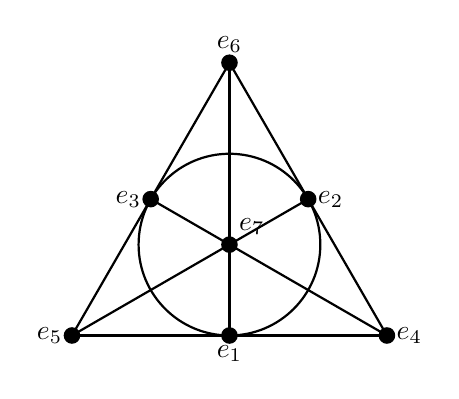
\begin{tikzpicture}[scale=2]
  \coordinate (A) at (0, 1.732);
  \coordinate (B) at (-1, 0);
  \coordinate (C) at (1, 0);
  \coordinate (D) at (0, 0);
  \coordinate (E) at (0.5, 0.866);
  \coordinate (F) at (-0.5, 0.866);
  \coordinate (O) at (0, 0.577);

  \draw[thick] (A) -- (B);
  \draw[thick] (B) -- (C);
  \draw[thick] (C) -- (A);
  \draw[thick] (A) -- (D);
  \draw[thick] (B) -- (E);
  \draw[thick] (C) -- (F);
  \draw[thick] (O) circle (0.577);

  \fill (A) circle (1.5pt) node[above]      {$e_6$};
  \fill (B) circle (1.5pt) node[left]       {$e_5$};
  \fill (C) circle (1.5pt) node[right]      {$e_4$};
  \fill (D) circle (1.5pt) node[below]      {$e_1$};
  \fill (E) circle (1.5pt) node[right]      {$e_2$};
  \fill (F) circle (1.5pt) node[left]       {$e_3$};
  \fill (O) circle (1.5pt) node[above right]{$e_7$};
\end{tikzpicture}
\caption{The Fano plane of $\mathrm{Im}(\mathbb{O})$, with labels consistent with Table~\ref{tab:oct}. Line orientations follow the signs of Table~\ref{tab:oct}; the incidence pattern itself is sign-blind. The seven Fano lines are: three sides $\{6,3,5\}$, $\{5,1,4\}$, $\{6,2,4\}$ (outer edges), three medians $\{6,7,1\}$, $\{5,7,2\}$, $\{4,7,3\}$, and the inscribed circle $\{1,2,3\}$.}
\label{fig:fano}
\end{figure}

\noindent Figure~\ref{fig:fano} displays the underlying Fano plane of $\mathrm{Im}(\mathbb{O})$ with the Fano-line labelling consistent with Table~\ref{tab:oct}; the generation triangle $K_3$ on $(g_1, g_2, g_3)$ is the complete graph on three vertices and is not drawn separately.

\section{Discussion}\label{sec:discuss}
\subsection{Relation to prior work}\label{sec:relation-prior-work}
Division-algebra approaches to flavor emphasize $\mathbb{O}$ and triality \cite{Baez2002,Boyle2020,Furey2018,Dixon1994book}.
We use $\mathbb{S}$ only as a probe of $\mathrm{Im}(\mathbb{O})$ through associator norms, and obtain a finite, rigid classification tied to Fano geometry.

The closest existing threads we are aware of are: the eigentheory of Cayley--Dickson multiplication operators by Biss--Christensen--Dugger--Isaksen~\cite{biss2009}, which studies the operator $M_a = L_{\bar a} L_a$ rather than associator-derived matrices; the relation graphs of the sedenion algebra developed by Guterman--Zhilina~\cite{guterman_zhilina2021}, which encode commutativity, orthogonality, and zero-divisor structure but not associator spectra; the finite-geometric encoding of Cayley--Dickson multiplication tables in $\mathrm{PG}(n-1,2)$ due to Saniga--Holweck--Pracna~\cite{saniga2015}, whose $\mathrm{PG}(3,2)$ realization of $\mathbb{S}$ is complementary to --- but distinct from --- ours; the graded classification of non-associativity types across the doubling chain due to Wilmot~\cite{wilmot2025structure}; and Moreno's characterization of alternative elements in Cayley--Dickson algebras~\cite{moreno2004}, which concerns within-level alternativity rather than cross-level probing. A separate physics-oriented thread studies $\mathbb{C} \otimes \mathbb{S}$ and Fano-plane idempotent decompositions for three-generation structure~\cite{gresnigt2019, gresnigt2023, gourlay_gresnigt2024}; that program uses $\mathbb{S}$ differently and is independent of our algebraic results.

Additional adjacent structural results include the baseline real-structure reference of Khalil and Yiu~\cite{khalil_yiu1997}, the large-annihilator analyses of Biss, Dugger, and Isaksen~\cite{biss_dugger_isaksen2008, biss_dugger_isaksen2007}, which refine the eigentheory of~\cite{biss2009} to study zero-divisor loci directly, and Zhilina's Part I on orthogonality graphs of doubly alternative zero divisors in real Cayley--Dickson algebras~\cite{zhilina2021} (the direct follow-up to~\cite{guterman_zhilina2021}). The subalgebra structure of $\mathbb{S}$ under $\mathrm{Aut}(\mathbb{S})$ was classified by Chan and Djokovic~\cite{chan_dokovic2006}, which provides the natural invariant-theoretic framework for refining our probe classification (cf. Open Problem~\ref{op:autS-invariance}).

Our contribution sits at the intersection of these threads: matrices built from associator data, spectral analysis of the resulting matrices, and recovery of Fano-plane structure from the classification.

\subsection{Related classifications}
\label{sec:related-classifications}

Guterman and Zhilina~\cite{guterman_zhilina2021} establish a bijection between the seven connected components of the orthogonality graph $\Gamma_O(\mathbb{S})$ and the seven Fano lines in $\mathrm{Im}(\mathbb{O})$ (their Theorem~4.15), where orthogonality is taken with respect to the standard trace-form inner product on $\mathbb{S}$, restricted to the set of zero divisors. The same paper establishes that the diameter of each connected component of $\Gamma_O(\mathbb{S})$ equals 3 (Corollary~4.10 combined with Theorem~4.11). The classified objects there are zero divisors; our classification, in contrast, partitions the eight probes $\{e_8, \ldots, e_{15}\}$ --- which are \emph{not} zero divisors --- into four classes. The partition cardinalities differ ($7$ vs.\ $4$), and the objects classified live in disjoint parts of $\mathbb{S}$ (zero divisors vs.\ unit-norm basis elements). The two classifications are complementary rather than comparable: both use Fano incidence as an organizing principle but apply it to distinct structural features. A follow-up by Zhilina~\cite{zhilina2024} establishes analogous diameter results for the commutativity graph of $\mathbb{S}$.
An interesting complementarity arises: Zhilina's analysis shows that basis elements with non-zero-divisor imaginary parts --- precisely our probes $\{e_8, \ldots, e_{15}\}$ --- appear as isolated vertices in the commutativity graph of $\mathbb{S}$, so the probes carry no structure at the level of second-order (commutativity) operations; yet at the level of third-order (associator) operations they exhibit the rich $(1, 3, 3, 1)$ stratification proved here. This order-dependent structural shift suggests that the non-associativity of $\mathbb{S}$ encodes information that its commutativity profile alone does not reveal.

Two 2024 works postdate v0.1 and further constrain the geometric picture. Reggiani~\cite{reggiani2024} proves that the normalized zero-divisor pair manifold $\mathcal{Z}(\mathbb{S}) \subset \mathbb{S} \times \mathbb{S}$ is isometric to the compact exceptional Lie group $G_2$ equipped with a naturally reductive left-invariant metric (refining the original topological identification of Moreno~\cite{moreno1998}), and exhibits a Riemannian submersion $\mathcal{Z}(\mathbb{S}) \to \mathrm{Gr}_{\mathbb{H}}(\mathbb{O}) = G_2/\mathrm{SO}(4)$ over the exceptional symmetric space of quaternion subalgebras of $\mathbb{O}$, with typical fibre locally isometric to a product of two round 3-spheres of distinct radii. This geometric realization of $G_2$ inside sedenion zero-divisor data is the natural companion to our algebraic Corollary~\ref{cor:g2-invariance}: both statements identify $G_2 = \mathrm{Aut}(\mathbb{O})$ as the relevant symmetry group, from different vantage points.

A subsequent preprint by Koebisu~\cite{koebisu2025} (version~2, March~2026) factorizes the determinant of left multiplication $L_v$ on $\mathbb{S}$ as $\det L_v = D_1(v)^4 \, D_2(v)^2$, with $D_1(v) = \|v\|^2$ and $D_2$ a $G_2$-invariant quartic; the vanishing of the normalized $D_2$ recovers the Stiefel manifold $V_2(\mathbb{R}^7) = G_2/\mathrm{SU}(2)$ as the zero-divisor locus (the original geometric result is Moreno~\cite{moreno1998}, and the Riemannian picture Reggiani~\cite{reggiani2024}). This refines the Reggiani realization at the determinantal level and identifies the same $G_2$-structure from a polynomial-invariant vantage point. Our probe matrices $A^{(k)}$ are scalar (norm-valued) rather than polynomial in the component data of sedenions, so the comparison with Koebisu's $D_2$ is structural (both objects are $G_2$-invariants built from sedenion bilinear data) rather than coefficient-level.

Wilmot~\cite{wilmot2025structure} classifies triples of basis elements in Cayley--Dickson algebras by associator/Moufang type, using a graded-construction framework with three associativity types (Theorem~2) and four non-associativity types (Theorem~5); the same preprint reduces the 84 primitive sedenion zero-divisors to 7 primitive triples indexed by Fano lines. A companion preprint~\cite{wilmot2025auto} introduces a 15-dimensional ``Fano volume'' visualizing the full subalgebra structure of $\mathbb{S}$ and derives the automorphism group $\mathrm{Aut}(\mathbb{S}) \cong G_2 \times S_3$ (matching Brown~\cite{brown1967}). Both Wilmot papers are 2025 arXiv preprints with no journal version at time of writing. Our classification is naturally indexed by pairs $(L_0, (g_1, g_2, g_3))$ (28 total configurations), while Wilmot's typology lives on unordered triads of basis elements with a canonical ordering $b < c < bc$; the two indexing sets are disjoint \emph{ex definitione}, and an explicit reduction map between the taxonomies is beyond the scope of this note. On $\mathbb{O}$, we invoke only the binary Fano vs.\ non-Fano distinction (Case D1 vs.\ Case D2 of Lemma~\ref{lem:quant}); Wilmot's finer non-associativity typology is not used here.

Saniga, Holweck, and Pracna~\cite{saniga2015} encode the multiplication table of Cayley--Dickson algebras as a graded sequence of finite-geometric configurations $C_N$: at level $N=3$ (octonions) the relevant configuration is the Pasch configuration $C_3 = (6_2, 4_3)$, and at level $N=4$ (sedenions) the configuration $C_4 = (10_3)$ is the Desargues configuration sitting in $\mathrm{PG}(3,2)$. Since we use sedenion probes only as external testers of the octonion Fano plane $\mathrm{PG}(2,2)$, our combinatorial ambient is $C_3$-level, not $C_4$-level. The classification presented here is independent of, and not derivable from, the Veldkamp-space structure of $C_4$ in~\cite{saniga2015}.

\paragraph{Further parallel threads.}
Several additional works provide indirect points of comparison.
Lopatin and Zubkov~\cite{lopatin_zubkov2024} provide a minimal separating and minimal generating set of polynomial $G_2$-invariants on tuples of octonions in odd characteristic (a separating set only, in characteristic~$2$); our associator norms $A^{(k)}_{ij}$ are scalar $G_2$-invariants on pairs of imaginary octonions (parameterized by the probe index $k$) and can in principle be expressed as polynomials in their generators, though we have not pursued this explicitly.
Yamazaki~\cite{yamazaki2008} constructs an explicit \emph{generalized} (not metric-positive) Lie 3-algebra on $\mathbb{O}$ with $G_2$ derivation algebra, motivated by $\mathcal{N}=2$ Chern--Simons matter theory on M2-branes; our probe construction is conceptually related but operates at the level of scalar associator norms rather than Lie 3-algebra structure.
De Marrais~\cite{de_marrais2000, de_marrais2004} (and the subsequent ``box-kite'' series) organizes the 42 primitive zero-divisor pairs of $\mathbb{S}$ into 7 ``box-kites'' indexed by Fano lines, with an implicit use of indices $k \in \{8, \ldots, 15\}$ as external probes in the Assessor construction; determining whether our $1+3+3+1$ partition refines, or is refined by, the box-kite stratification (and whether Edge/Hub triples align with the $S_3$-Brown orbits on basis elements) is an open structural question (see Open Problem~\ref{op:boxkites} in \S\ref{sec:open}).

To put these 7-fold stratifications of $\mathbb{S}$ side by side, Table~\ref{tab:stratifications} collects the structures from the most directly relevant antecedents.

\begin{table}[h]
\centering
\caption{Four 7-fold stratifications of sedenion structure, each indexed by the seven Fano lines of $\mathrm{Im}(\mathbb{O})$.}
\label{tab:stratifications}
\begin{tabular}{l|l|l|l}
\toprule
Source & Count & Decomposition & Objects indexed \\
\midrule
Wilmot~\cite{wilmot2025structure} & $84 = 12 \cdot 7$ & Primitive zero-divisor triples & Zero-divisor triples \\
de Marrais~\cite{de_marrais2000} & $42 = 6 \cdot 7$ & Primitive zero-divisor pairs (Assessors) & Zero-divisor pairs \\
This paper & $28 = 4 \cdot 7$ & Unit-probe configurations $(L_0, (g_1, g_2, g_3))$ & Configurations \\
Wilmot~\cite{wilmot2025structure} & $7 = 1 \cdot 7$ & Primitive triples (Fano-line representatives) & Fano lines \\
\bottomrule
\end{tabular}
\end{table}

De Marrais stratifies the zero-divisor set $\mathcal{Z}(\mathbb{S})$ via six zero-divisor pairs per Fano line; the present work stratifies the complementary unit-probe configuration space $\mathfrak{U} = \{(L_0, (g_1, g_2, g_3))\}$ via four configurations per Fano line. The two stratifications are complementary (zero-divisor side vs.\ invertible-unit side of $\mathbb{S}$), and we are not aware of a previous tabulation placing them alongside each other.

Finally, Dray and Manogue~\cite{dray_manogue1998} analyze spectra of $3 \times 3$ Hermitian octonionic matrices arising in the exceptional Jordan algebra $J_3(\mathbb{O})$; their construction uses octonionic matrix entries rather than scalar associator norms, but the general paradigm ``$3 \times 3$ spectral problem derived from associator / non-associativity data'' has precedent there.

\subsection{What we do \emph{not} claim}\label{sec:nonclaims}
We do not claim that $\mathbb{S}$ is realized as an internal symmetry algebra of fermions, nor that the classification implies a unique physical model.

\subsection{Open problems}\label{sec:open}
\begin{enumerate}
  \item Classify the analogue for split-octonions (signature $(4,4)$) and compare eigenpatterns.
  \item Is the $1+3+3+1$ multiset partition canonically $\mathrm{Aut}(\mathbb{O})$-equivariant on labeled probes (as a decomposition into four indexed families), or only preserved as an unordered decomposition into four blocks?
  \item Extend the classification to the trigintaduonions $\mathbb{T} = \mathbb{A}_5$ (the next Cayley--Dickson algebra, of dimension $32$). Concretely, form the analogous associator-probe matrices using the $16$ basis vectors in the doubled half as probes, and determine whether the resulting eigenpattern refines $1 + 3 + 3 + 1$ by an extra block consistent with Wilmot's fourth non-associativity type~\cite{wilmot2025structure, wilmot2025auto}; the entry quantization (Lemma~\ref{lem:quant}) will likely fail at this level, requiring a finer classification of associator values beyond $\{0, 2\}$.
  \item \label{op:autS-invariance} Is the classification invariant under the full $\mathrm{Aut}(\mathbb{S}) = G_2 \times S_3$ (cf.\ Corollary~\ref{cor:g2-invariance})? Equivalently, does the Brown $S_3$ factor~\cite{brown1967} permute the Edge and Hub triples $\{e_{8+\ell} : \ell \in L_0\}$ and $\{e_{8+g_i} : i \in \{1,2,3\}\}$ within their respective blocks, or across them? A positive answer would identify our partition as a function of $S_3$-orbits of probes.
  \item \label{op:boxkites} Compare the probe-to-class mapping with de Marrais' box-kite stratification~\cite{de_marrais2000, de_marrais2004} of sedenion zero-divisors. Since box-kites are indexed by Fano lines and partition the Assessor construction into seven 6-cycle orbits, a direct comparison requires identifying the $(L_0, (g_1, g_2, g_3))$ parameters with box-kite indices; this would position our $1+3+3+1$ classification within the classical zero-divisor combinatorics of $\mathbb{S}$.
  \item The $224$-configuration space $\mathfrak{U} \times \{\text{probes}\}$ (where $\mathfrak{U} = \{(L_0, (g_1, g_2, g_3))\}$) is a $G_2$-equivariant collection of scalar invariants on triples of octonions. Expressing the four spectral classes as specific polynomial combinations in the minimal generating set of $G_2$-invariants due to Lopatin and Zubkov~\cite{lopatin_zubkov2024} would place our classification within the invariant-theoretic framework for tuples of octonions and may reveal underlying Casimir-type structure.
\end{enumerate}

\FloatBarrier
\appendix
\section{Octonion multiplication signs (Cayley--Dickson)}\label{app:mult}
Table~\ref{tab:oct} lists $e_ie_j$ as $\pm e_k$ in the standard Cayley--Dickson basis adopted throughout.

\begin{table}[ht]
\centering
\small
\begin{tabular}{r|rrrrrrrr}
\toprule
      & $e_0$ & $e_1$ & $e_2$ & $e_3$ & $e_4$ & $e_5$ & $e_6$ & $e_7$\\\hline
$e_0$ & $+e_0$ & $+e_1$ & $+e_2$ & $+e_3$ & $+e_4$ & $+e_5$ & $+e_6$ & $+e_7$\\
$e_1$ & $+e_1$ & $-e_0$ & $+e_3$ & $-e_2$ & $+e_5$ & $-e_4$ & $-e_7$ & $+e_6$\\
$e_2$ & $+e_2$ & $-e_3$ & $-e_0$ & $+e_1$ & $+e_6$ & $+e_7$ & $-e_4$ & $-e_5$\\
$e_3$ & $+e_3$ & $+e_2$ & $-e_1$ & $-e_0$ & $+e_7$ & $-e_6$ & $+e_5$ & $-e_4$\\
$e_4$ & $+e_4$ & $-e_5$ & $-e_6$ & $-e_7$ & $-e_0$ & $+e_1$ & $+e_2$ & $+e_3$\\
$e_5$ & $+e_5$ & $+e_4$ & $-e_7$ & $+e_6$ & $-e_1$ & $-e_0$ & $-e_3$ & $+e_2$\\
$e_6$ & $+e_6$ & $+e_7$ & $+e_4$ & $-e_5$ & $-e_2$ & $+e_3$ & $-e_0$ & $-e_1$\\
$e_7$ & $+e_7$ & $-e_6$ & $+e_5$ & $+e_4$ & $-e_3$ & $-e_2$ & $+e_1$ & $-e_0$\\
\bottomrule
\end{tabular}
\caption{Cayley--Dickson octonion products $e_ie_j$.}\label{tab:oct}
\end{table}

\section{The 28 probe-to-class configurations}
\label{app:configs}

Table~\ref{tab:summary} summarizes the structural pattern common to all $28$ rows: one probe per class, with class assignment determined by the relationship between $k - 8$ and $(L_0, (g_1, g_2, g_3))$.

\begin{table}[h]
\centering
\caption{Summary of the probe-to-class assignment (one row per class), uniformly across all $28$ configurations.}
\label{tab:summary}
\begin{tabular}{l|l|l}
\toprule
Class & Condition on $k$ & Eigenvalues of $A^{(k)}$ \\
\midrule
Democratic & $k = 8$ & $\{4, -2, -2\}$ \\
Edge & $k \in \{8 + \ell : \ell \in L_0\}$ & $\{2, 0, -2\}$ \\
Hub & $k \in \{8 + g_i : i = 1, 2, 3\}$ & $\{2\sqrt{2}, 0, -2\sqrt{2}\}$ \\
Zero & $k = 8 + g_4$ & $\{0, 0, 0\}$ \\
\bottomrule
\end{tabular}
\end{table}

The full configuration-by-configuration assignment is tabulated below (Table~\ref{tab:full-configs}) for completeness and to facilitate independent verification.
The Democratic class always contains probe $e_8$ and is omitted from the full table columns.

\begin{table}[htbp]
\centering
\footnotesize
\caption{The 28 configurations $(L_0, (g_1, g_2, g_3))$ and their probe-to-class assignments. Democratic $= \{e_8\}$ in every row (omitted). Probe indices $k$ are displayed; the corresponding probe is $e_k$.}
\label{tab:full-configs}
\begin{tabular}{l|l|l|l|l|l}
\hline
$L_0$ & $(g_1, g_2, g_3)$ & $g_4$ & Edge & Hub & Zero \\
\hline
$\{1,2,3\}$ & $(4,5,6)$ & $7$ & $\{9,10,11\}$ & $\{12,13,14\}$ & $15$ \\
$\{1,2,3\}$ & $(4,5,7)$ & $6$ & $\{9,10,11\}$ & $\{12,13,15\}$ & $14$ \\
$\{1,2,3\}$ & $(4,6,7)$ & $5$ & $\{9,10,11\}$ & $\{12,14,15\}$ & $13$ \\
$\{1,2,3\}$ & $(5,6,7)$ & $4$ & $\{9,10,11\}$ & $\{13,14,15\}$ & $12$ \\
\hline
$\{1,4,5\}$ & $(2,3,6)$ & $7$ & $\{9,12,13\}$ & $\{10,11,14\}$ & $15$ \\
$\{1,4,5\}$ & $(2,3,7)$ & $6$ & $\{9,12,13\}$ & $\{10,11,15\}$ & $14$ \\
$\{1,4,5\}$ & $(2,6,7)$ & $3$ & $\{9,12,13\}$ & $\{10,14,15\}$ & $11$ \\
$\{1,4,5\}$ & $(3,6,7)$ & $2$ & $\{9,12,13\}$ & $\{11,14,15\}$ & $10$ \\
\hline
$\{1,6,7\}$ & $(2,3,4)$ & $5$ & $\{9,14,15\}$ & $\{10,11,12\}$ & $13$ \\
$\{1,6,7\}$ & $(2,3,5)$ & $4$ & $\{9,14,15\}$ & $\{10,11,13\}$ & $12$ \\
$\{1,6,7\}$ & $(2,4,5)$ & $3$ & $\{9,14,15\}$ & $\{10,12,13\}$ & $11$ \\
$\{1,6,7\}$ & $(3,4,5)$ & $2$ & $\{9,14,15\}$ & $\{11,12,13\}$ & $10$ \\
\hline
$\{2,4,6\}$ & $(1,3,5)$ & $7$ & $\{10,12,14\}$ & $\{9,11,13\}$ & $15$ \\
$\{2,4,6\}$ & $(1,3,7)$ & $5$ & $\{10,12,14\}$ & $\{9,11,15\}$ & $13$ \\
$\{2,4,6\}$ & $(1,5,7)$ & $3$ & $\{10,12,14\}$ & $\{9,13,15\}$ & $11$ \\
$\{2,4,6\}$ & $(3,5,7)$ & $1$ & $\{10,12,14\}$ & $\{11,13,15\}$ & $9$ \\
\hline
$\{2,5,7\}$ & $(1,3,4)$ & $6$ & $\{10,13,15\}$ & $\{9,11,12\}$ & $14$ \\
$\{2,5,7\}$ & $(1,3,6)$ & $4$ & $\{10,13,15\}$ & $\{9,11,14\}$ & $12$ \\
$\{2,5,7\}$ & $(1,4,6)$ & $3$ & $\{10,13,15\}$ & $\{9,12,14\}$ & $11$ \\
$\{2,5,7\}$ & $(3,4,6)$ & $1$ & $\{10,13,15\}$ & $\{11,12,14\}$ & $9$ \\
\hline
$\{3,4,7\}$ & $(1,2,5)$ & $6$ & $\{11,12,15\}$ & $\{9,10,13\}$ & $14$ \\
$\{3,4,7\}$ & $(1,2,6)$ & $5$ & $\{11,12,15\}$ & $\{9,10,14\}$ & $13$ \\
$\{3,4,7\}$ & $(1,5,6)$ & $2$ & $\{11,12,15\}$ & $\{9,13,14\}$ & $10$ \\
$\{3,4,7\}$ & $(2,5,6)$ & $1$ & $\{11,12,15\}$ & $\{10,13,14\}$ & $9$ \\
\hline
$\{3,5,6\}$ & $(1,2,4)$ & $7$ & $\{11,13,14\}$ & $\{9,10,12\}$ & $15$ \\
$\{3,5,6\}$ & $(1,2,7)$ & $4$ & $\{11,13,14\}$ & $\{9,10,15\}$ & $12$ \\
$\{3,5,6\}$ & $(1,4,7)$ & $2$ & $\{11,13,14\}$ & $\{9,12,15\}$ & $10$ \\
$\{3,5,6\}$ & $(2,4,7)$ & $1$ & $\{11,13,14\}$ & $\{10,12,15\}$ & $9$ \\
\hline
\end{tabular}
\end{table}

Each row exhibits the multiplicity pattern $1 + 3 + 3 + 1 = 8$ predicted by Theorem~\ref{thm:classification}; every assignment agrees with the case analysis in the proof of Theorem~\ref{thm:strong}.

\clearpage
\section*{Acknowledgments}

\begin{sloppypar}
Computational verification was performed with exact integer Cayley--Dickson multiplication (Python package \texttt{quantum-foundations}, import path \path{quantum_foundations.sedenion}; Jupyter notebooks and \path{COMPANION.md} under \path{papers/sedenion-associator-probe/}).
The code is publicly available at \url{https://github.com/bartrosa/quantum-foundations} and archived at \url{https://doi.org/10.5281/zenodo.19694537}~\cite{rosa2026code}, with the specific state verifying the results of this paper pinned to git tag \path{v1.0-paper-A1-sedenion}.
\end{sloppypar}

\clearpage
\bibliographystyle{plain}
\bibliography{references}

\end{document}
